%
% Copyright (c) 2017 Radoslaw Kujawa.
% All rights reserved.
%
% Redistribution and use in source and binary forms, with or without
% modification, are permitted provided that the following conditions
% are met:
%
% 1. Redistributions of source code must retain the above copyright
%    notice, this list of conditions and the following disclaimer.
% 2. Redistributions in binary form must reproduce the above copyright
%    notice, this list of conditions and the following disclaimer in the
%    documentation and/or other materials provided with the distribution.
%
% THIS SOFTWARE IS PROVIDED BY RADOSLAW KUJAWA (THE AUTHOR) AND CONTRIBUTORS
% ``AS IS'' AND ANY EXPRESS OR IMPLIED WARRANTIES, INCLUDING, BUT NOT LIMITED
% TO, THE IMPLIED WARRANTIES OF MERCHANTABILITY AND FITNESS FOR A PARTICULAR
% PURPOSE ARE DISCLAIMED.  IN NO EVENT SHALL THE AUTHOR OR CONTRIBUTORS
% BE LIABLE FOR ANY DIRECT, INDIRECT, INCIDENTAL, SPECIAL, EXEMPLARY, OR
% CONSEQUENTIAL DAMAGES (INCLUDING, BUT NOT LIMITED TO, PROCUREMENT OF
% SUBSTITUTE GOODS OR SERVICES; LOSS OF USE, DATA, OR PROFITS; OR BUSINESS
% INTERRUPTION) HOWEVER CAUSED AND ON ANY THEORY OF LIABILITY, WHETHER IN
% CONTRACT, STRICT LIABILITY, OR TORT (INCLUDING NEGLIGENCE OR OTHERWISE)
% ARISING IN ANY WAY OUT OF THE USE OF THIS SOFTWARE, EVEN IF ADVISED OF THE
% POSSIBILITY OF SUCH DAMAGE.
%
% 
\documentclass[dvipsnames,table]{beamer}
\usepackage{polski}

\usetheme{Rochester}
\usecolortheme{orchid}

\usepackage{listings}
\usepackage{ucs}
\usepackage[utf8x]{inputenc}
\usepackage{wasysym}
\usepackage[normalem]{ulem}
\usepackage{amsmath}
\usepackage{hyperref}
\usepackage{tikzsymbols}

\setbeamertemplate{navigation symbols}{}
\setbeamertemplate{caption}[numbered]
\setbeamerfont{caption}{size=\scriptsize}
\setbeamercolor{framenote}{bg=OSEC-red!25}
\setbeamercolor{rednote}{bg=Red!25}
\setbeamercolor{palette primary}{use=structure,fg=white,bg=OSEC-red}
\setbeamercolor{palette secondary}{use=structure,fg=white,bg=OSEC-red2}

\setbeamertemplate{itemize item}{\scriptsize\raise1pt\hbox{\donotcoloroutermaths$\blacktriangleright$}}
\setbeamertemplate{itemize subitem}{\tiny\raise1pt\hbox{\donotcoloroutermaths$\bullet$}}
\setbeamertemplate{itemize subsubitem}{\tiny\raise1pt\hbox{\donotcoloroutermaths{--}}}

\setbeamertemplate{enumerate item}{\insertenumlabel.}
\setbeamertemplate{enumerate subitem}{\insertenumlabel.\insertsubenumlabel}
\setbeamertemplate{enumerate subsubitem}{\insertenumlabel.\insertsubenumlabel.\insertsubsubenumlabel}
\setbeamertemplate{enumerate mini template}{\insertenumlabel}

\setbeamercolor{itemize item}{fg=OSEC-red, bg=OSEC-red}
\setbeamercolor{itemize subitem}{fg=OSEC-red, bg=OSEC-red}
\setbeamercolor{itemize subsubitem}{fg=OSEC-red, bg=OSEC-red}

\setbeamercolor{section number projected}{fg=white,bg=OSEC-red}
\setbeamercolor{subsection number projected}{fg=white,bg=OSEC-red}
\setbeamercolor{button}{bg=OSEC-red,fg=white}

\setbeamertemplate{section in toc}[circle]
\setbeamertemplate{subsection in toc}[square]

\definecolor{OSEC-red}{RGB}{160,29,44}
\definecolor{OSEC-red2}{RGB}{177,76,12}
\hypersetup{colorlinks=true,linkcolor=white,urlcolor=OSEC-red}

\setlength{\tabcolsep}{8pt}
\renewcommand{\arraystretch}{1.2}

\newcommand{\tri}{$\triangleright$ }

\title{OpenStack Neutron -- Software Defined Networking w prywatnych chmuarch}
\author{Radosław Kujawa -- radoslaw.kujawa@osec.pl}
\institute{OSEC}

\begin{document}

\begin{frame}
	\titlepage
\end{frame}

\begin{frame}
\frametitle{OpenStack + Neutron}
\begin{itemize}
	\item OpenStack -- nie tylko wirtualizacja CPU i pamięci, ale też pamięci masowej i sieci.
	\item Neutron -- zarządzanie infrastrukturą sieciową L2/L3 i usługami sieciowymi dla potrzeb chmury.
	\item Różne potrzeby klientów -- konieczność stworzenia bardzo elastycznego mechanizmu wirtualizacji sieci.
	\item Współpraca z zewnętrzną infrastrukturą sieciową.
\end{itemize}
\end{frame}

\begin{frame}
\frametitle{Funkcjonalności Neutrona}
\begin{itemize}
	\item Warstwa 2 - sterowniki ML2 (,,mechanism driver'' np. Open vSwitch).
	\item Warstwa 3 - Layer 3 agents (routing, DHCP\dots).
	\item Foo as a Service
	\begin{itemize}
		\item Firewall as a Service.
		\item VPN as a Service.
		\item Load balancer as a Service.
		\item \dots 
	\end{itemize}
\end{itemize}
\end{frame}

\begin{frame}
\frametitle{Architektura sieci w Neutronie}
\begin{itemize}
	\item Założenie: każdy projekt w OpenStack może posiadać zupełnie odrębne, niezależne sieci (oddzielna warstwa 2).
	\item Projekty w OpenStack mogą o sobie na wzajem nic nie wiedzieć.
	\item Sieci prywatne i publiczne.
	\item Możliwość routowania między sieciami.
	\item Mechanizmy separacji sieci (,,type driver''):
	\begin{itemize}
		\item VLAN.
		\item VXLAN.
		\item GRE.
		\item Geneve.
		\item \dots
	\end{itemize}
\end{itemize}
\end{frame}

\begin{frame}
\frametitle{Architektura z centralnym punktem dostępu do sieci zewnętrznej}
\begin{itemize}
	\item Domyślna architektura idealna pod potrzeby ,,hostingowe''. 
	\item Prostota wdrożenia.
	\item Izolacja projektów -- tunelowanie sieci prywatnych.
	\item Jeden punkt styku z siecią fizyczną na węźle sieciowym.
	\item Maszyny wirtualne posiadają interfejsy w sieciach prywatnych (,,projektowych'').
	\item Instancje maszyn wirtualnych {\em nie mogą} posiadać interfejsów przyłączonych bezpośrednio do sieci fizycznej (brak odp. bridge'y na węzłach obliczeniowych).
\end{itemize}
\end{frame}

\begin{frame}
\frametitle{Architektura z centralnym punktem dostępu do sieci zewnętrznej}
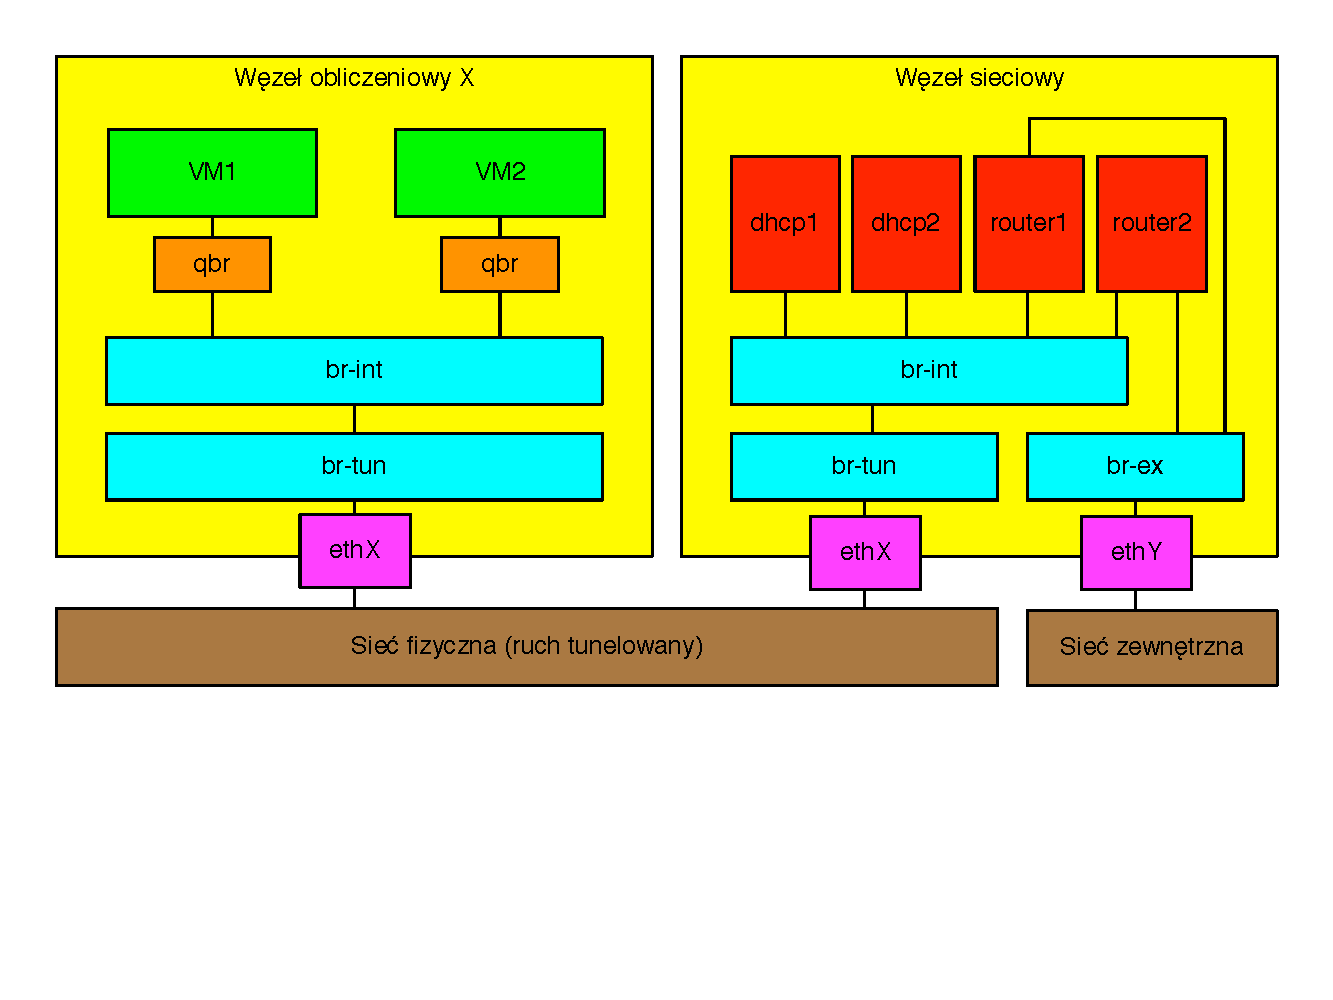
\includegraphics[width=1.00\textwidth]{img-neutron-tenantonly.pdf}
\end{frame}

\begin{frame}
\frametitle{Architektura z dostępem do sieci zewnętrznej na każdym węźle obliczeniowym}
\begin{itemize}
	\item Alternatywny sposób konfiguracji Neutrona.
	\item Może być bardziej skomplikowany we wdrożeniu.
	\item Sieci ,,provider''.
	\item Type driver {\tt flat} -- dostęp maszyny wirtualnej do sieci fizycznej.
	\item Type driver {\tt vlan}/{\tt vxlan} -- dostęp do odseparowanego segmentu sieci fizycznej.
	\item Separacja prywatnych sieci projektowych w dalszym ciągu możliwa.
\end{itemize}
\end{frame}

\begin{frame}
	\frametitle{Architektura z dostępem do sieci zewnętrznej na każdym węźle obliczeniowym}
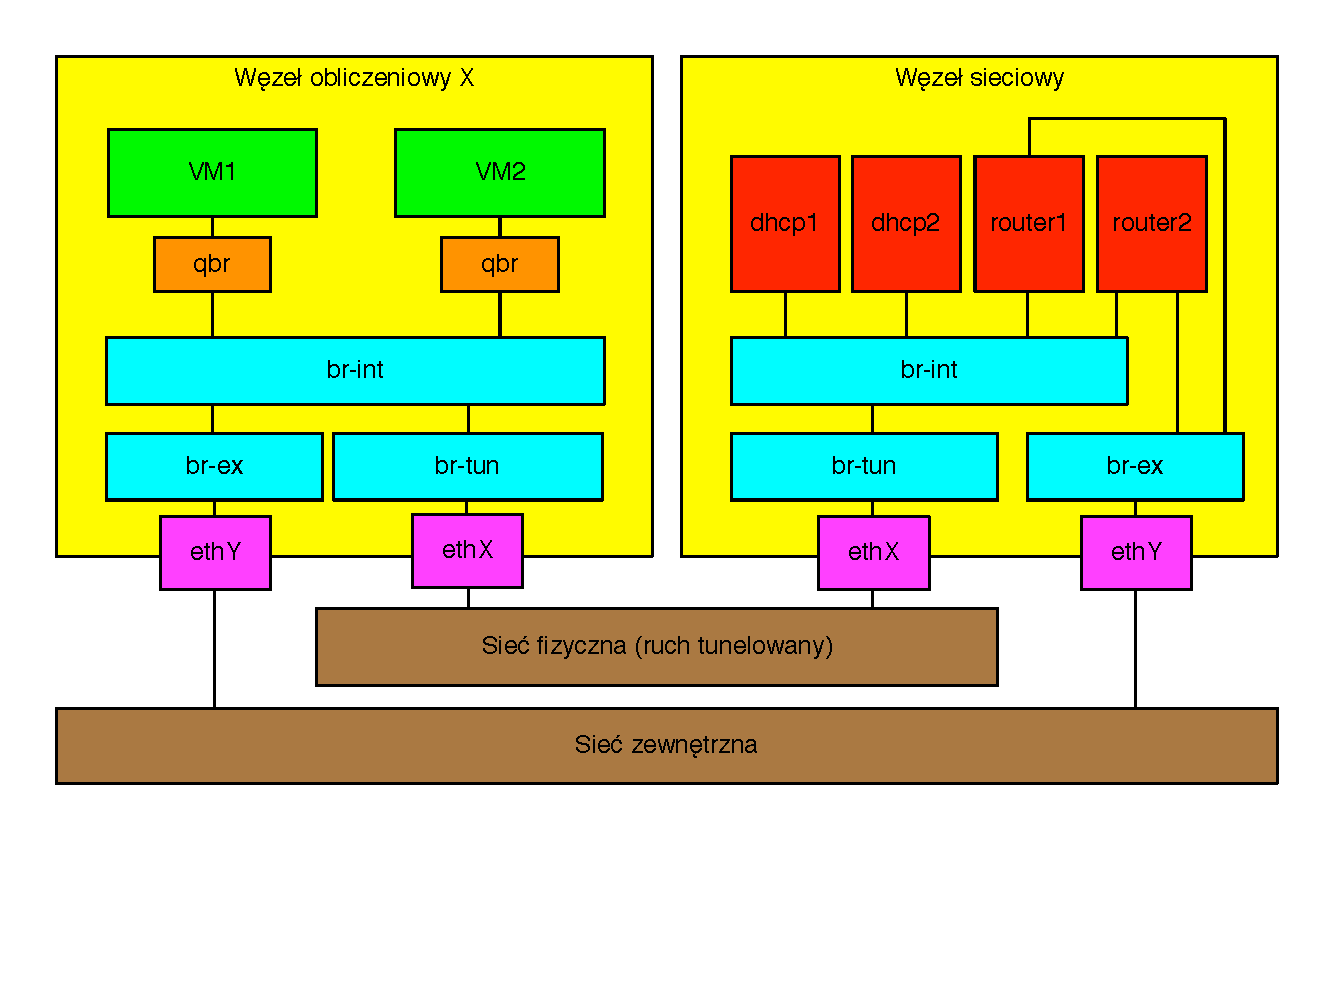
\includegraphics[width=1.00\textwidth]{img-neutron-provider.pdf}
\end{frame}

\begin{frame}
\frametitle{Integracja Neutrona z zewnętrznymi rozwiązaniami}
\begin{itemize}
	\item API REST oferowane przez Neutron.
	\item Pluginy do zarządzania warstwą 2 i 3.
	\begin{itemize}
		\item Cisco Nexus.
		\item Juniper.
		\item VMware NSX.
		\item \dots
	\end{itemize}
	\item Integracja z kontrolerami SDN i NFV.
	\begin{itemize}
		\item OpenContrail.
		\item OpenDaylight.
		\item \dots
	\end{itemize}
	\item Możliwość wykorzystania Neutrona z Red Hat Virtualization.
\end{itemize}
\end{frame}

\begin{frame}
\frametitle{Neutron a zastosowania telco/NFV}
\begin{itemize}
	\item Wymagany bezpośredni dostęp do sieci fizycznej.
	\item Jak najniższe opóźnienia w transmisji pakietów.
	\begin{itemize}
		\item PCI passthrough.
		\item SR-IOV (karty Intel/Mellanox/QLogic, od OpenStack Juno).
		\begin{itemize}
			\item ML2 driver {\tt sriovnicswitch} -- sieci VLAN i flat.
		\end{itemize}
		\item DPDK (Open vSwitch data path, od OpenStack Mitaka).
	\end{itemize}
	\item Service chaining (OpenStack Ocata) -- obecnie wymaga Open vSwitch.
\end{itemize}
\end{frame}

\begin{frame}
\frametitle{Demonstracja}
\begin{itemize}
	\item Kilka przykładów konfiguracji z wykorzystaniem konfiguracji sieci ,,provider''. 
	\begin{itemize}
		\item Demo: utworzenie sieci zewnętrznych.
		\item Demo: utworzenie maszyny wirtualnej z interfejsem w sieci zewnętrznej.
		\item Demo: utworzenie sieci prywatnej.
		\item Demo: utworzenie maszyny wirtualnej z interfejsesm w sieci prywatnej.
		\item Demo: utworzenie routera między siecią prywatną i zewnętrzną.
		\item Demo: pływający adres IPv4.
	\end{itemize}
\end{itemize}
\end{frame}

\begin{frame}
	\frametitle{Podsumowując}
\begin{itemize}
	\item Neutron jest elastyczny -- możesz zaimplementować taką architekturę sieci jaka jest Ci potrzebna.
	\item Możliwość samodzielnego rozszerzania Neutrona przez pluginy.
	\item Wsparcie dla nowoczesnych standardów na różnych poziomach sieci -- IPv6, SR-IOV, DPDK, itd.
	\item Jeśli masz inne potrzeby\dots
	\item Chcesz skonsultować swoją architekturę\dots
	\item Pragniesz zbudować środowisko {\em proof of concept}...
	\item Potrzebujesz nowego pluginu\dots
	\item Odezwij się do nas! 
\end{itemize}
\end{frame}

\begin{frame}
\frametitle{Koniec\ldots}
\begin{center}

\includegraphics[scale=0.5]{img-oseclogo.png}

Dziękuje!

Czy są pytania?

\end{center}
\end{frame}
\end{document}

